%課題研究レジュメテンプレート ver. 1.1

\documentclass[uplatex]{jsarticle}
\usepackage[top=20mm,bottom=20mm,left=20mm,right=20mm]{geometry}
\usepackage[T1]{fontenc}
\usepackage{txfonts}
\usepackage{wrapfig}
\usepackage[expert,deluxe]{otf}
\usepackage[dvipdfmx,hiresbb]{graphicx}
\usepackage[dvipdfmx]{hyperref}
\usepackage{pxjahyper}
\usepackage{here}



\makeatletter
  \renewcommand{\section}{%
    \if@slide\clearpage\fi
    \@startsection{section}{1}{\z@}%
    {\Cvs \@plus.5\Cdp \@minus.2\Cdp}% 前アキ
    {.5\Cvs \@plus.3\Cdp}% 後アキ
    %{\normalfont\Large\headfont\raggedright}}
    {\normalfont\raggedright}}

  \renewcommand{\subsection}{\@startsection{subsection}{2}{\z@}%
    {\Cvs \@plus.5\Cdp \@minus.2\Cdp}% 前アキ
    {.5\Cvs \@plus.3\Cdp}% 後アキ
    %{\normalfont\large\headfont}}
    {\normalfont}}

  \renewcommand{\subsubsection}{\@startsection{subsubsection}{3}{\z@}%
    {\Cvs \@plus.5\Cdp \@minus.2\Cdp}%
    {\z@}%
    %{\normalfont\normalsize\headfont}}
    {\normalfont}}
\makeatother
%ここから上を編集する必要はない.





\title{\vspace{-14mm}GitHubのソフトウェア開発における貢献度分析}
\author{PMコース 矢吹研究室 1342100 春川 直幸}
\date{}%日付を入れる必要はない.
\pagestyle{empty}%ページ番号は振らない.
\begin{document}
\maketitle





\section{研究の背景}

ソフトウェア開発では,複数のメンバが同時に開発を行うため,ファイルの最新バージョンが分からなくなる,同一ファイルに対する変更が競合する等の問題が発生する.このような問題を解決するため,バージョン管理システムを用いる\cite{ikeda2014}.バージョン管理システムとは,変更履歴を管理するシステムのことである.具体的にはソフトウェアのソースコードを書き足したり,変更したりする過程を記録していき,特定の段階まで戻ったり,誤って消してしまったファイルを復活させたりなど,ソフトウェア開発の現場において無くてはならない機能である\cite{otuka2014}.

バージョン管理システムを提供するサービスに,GitHubがある.
GitHubではgit logコマンドというものがある.git logコマンドとは,リポジトリのコミットされたログを確認できるコマンドである.誰がいつコミットやマージをしてどのような差分を発生したのか確認できる.\cite{otuka2014}
このgit logコマンドを解析することにより,コミットによる開発者の貢献度を求め,GitHubでのソフトウェア開発でもパレートの法則が成り立つのか調査する.

\section{研究の目的}

GitHubを用いたソフトウェア開発プロジェクトにおいて,コミット数によるプロジェクトへの貢献度を可視化し,結果を分析する.

\section{プロジェクトマネジメントとの関連}

コミットによるプロジェクトの貢献度を分析しパレート図を作成することにより,GitHub を用いたソフトウェア開発プロジェクトでの,管理上の優先度を明示させる.
これはプロジェクトマネジメントの知識エリアにおいて,品質マネジメントに該当する.


\section{研究の方法}


本研究は2段階に分かれる.
\begin{enumerate}
\item シェル(Shell)を使用し,GitHub上のプロジェクトから,開発者数とコミット回数を調査する.
\item 調査したデータの分析をする.
\end{enumerate}


調査したデータの分析は,デシル分析で行う.
デシル分析とは,購買履歴データをもとに全顧客の購入金額を高い順に10等分して、各ランク(デシル1~10)の購入比率や売上高構成比を算出する主にマーケティングで使用する分析方法のことである\cite{decyl01}.
今回はデシル分析でコミット数の多い順に10等分して,各ランク(デシル1~デシル10)のコミット比率を算出し,コミット貢献度を明らかにする.



\section{現在の進捗状況}



GitHub上の10個のプロジェクトから,プロジェクトの開発者数、コミット数を調査し,デシル分析を行った.

開発者人数は最少1人,最大3503人だった.コミット数は最小1,最大54421だった.

10件のプロジェクトをデシル分析し平均を算出した.結果は,図1である.図1をグラフ化したものが図2になる.分析結果から,デシル1の構成比が88%になっており,約9割の成果は1割の開発者によって生み出されていることがわかった.

こうなった要因として調査した10件のプロジェクトでオーナーのコミット数が一位だったことが関係していると考える.コミット数が一位だった開発者の構成比の平均を求めた結果,42.4%だった.

このことから,GitHubにおけるソフトウェア開発では,パレートの法則とは若干違う結果になっていると言えるであろう.

\begin{wrapfigure}[20]{t}{8cm}
\vspace*{-\intextsep}
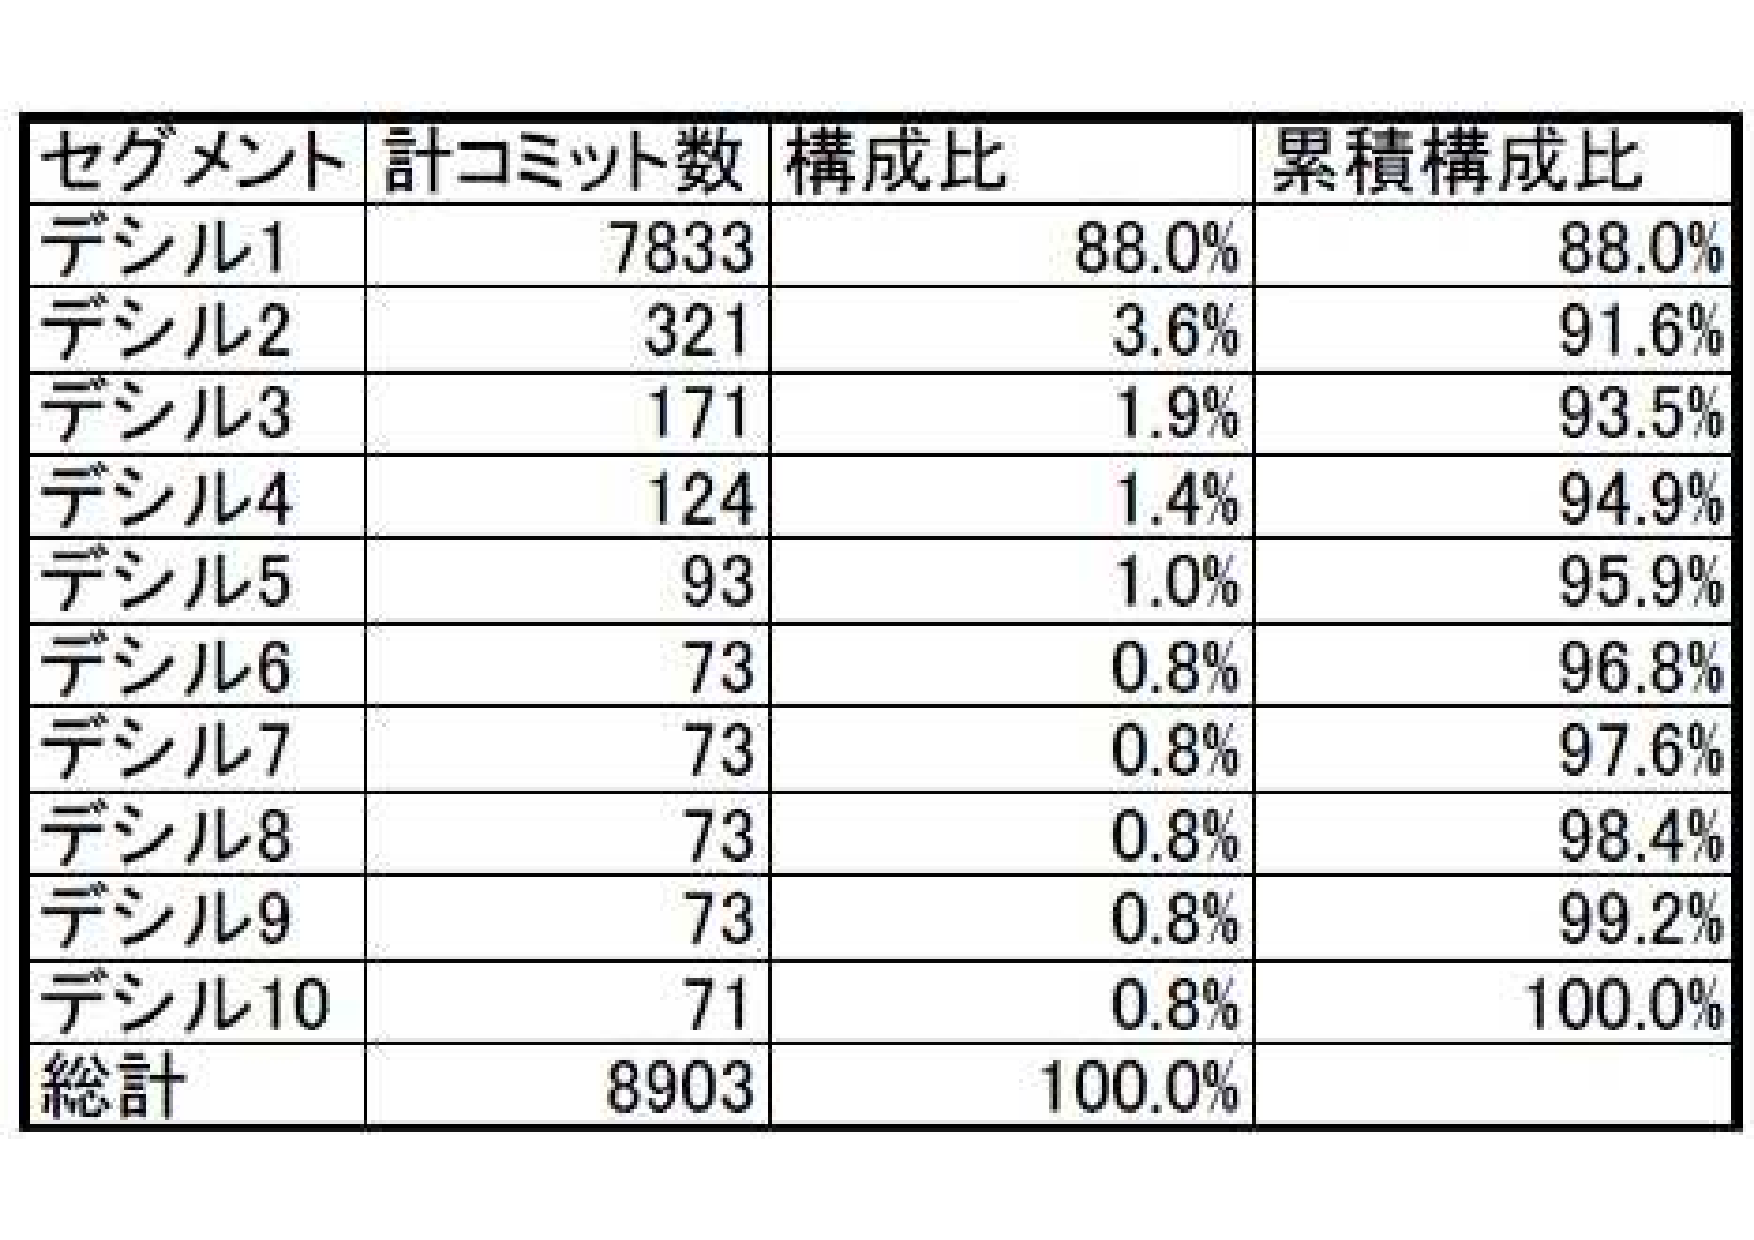
\includegraphics[width=7cm]{t2.pdf}
\caption{デシル分析 表}\label{デシル分析 表}

\vspace*{-\intextsep}
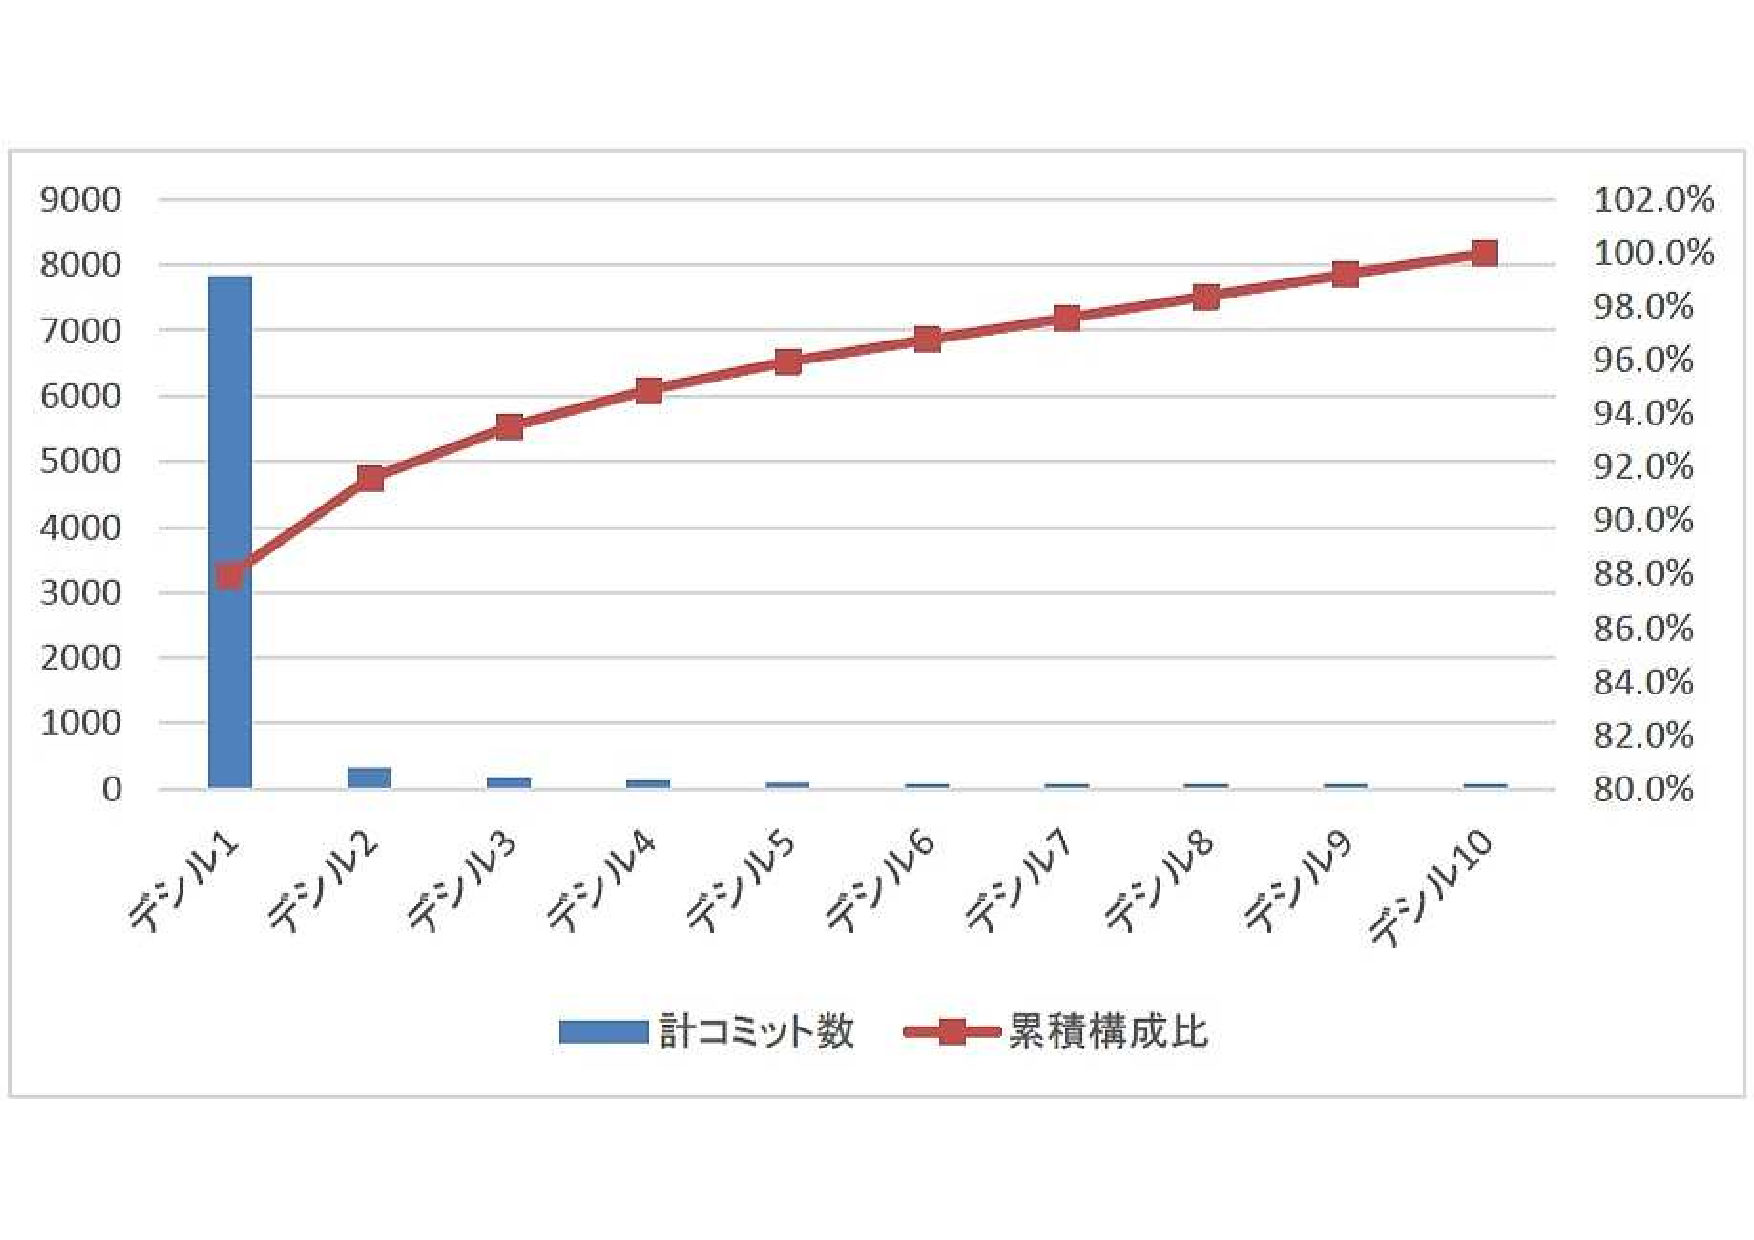
\includegraphics[width=7cm]{g2.pdf}
\caption{デシル分析 グラフ}\label{デシル分析 グラフ}
\end{wrapfigure}

\section{今後の計画}

以下のように研究を進める計画である.

\begin{enumerate}
\item データを自動で集められるように環境を整える. 
\item 調査対象となるプロジェクトの数を増やしたり,他の分析手法も用いて分析を行う.
\item 論文の執筆を行う.

\end{enumerate}

\bibliographystyle{junsrt}
\bibliography{biblio}%「biblio.bib」というファイルが必要.

\end{document}
